%%%%%%%%%%%%%%%%%%%%%%%% NOTES TO CONTRIBUTORS %%%%%%%%%%%%%%%%%%%%%%%%%%%%%%%%%
% - try to stick to a minimal package set unless you need them. In other words,
% don't use packages you don't understand simply because you're used to using
% them.
% - $$ eqn $$ is less universal than \[ eqn \] or \begin{equation} eqn \end{eqn}
% - Don't use the math environment just to center things. That's what the center
% environment is for.
% - If you have other stylistic guidelines you want other people to keep in
% mind, put them here


% In the future we may want to break this into many subfiles (see the subfiles
% package) so that we're not all working on a single monolithic document that
% takes a long time to compile.

\documentclass[a4paper, 11pt, oneside]{book}

\usepackage{a4wide}
\usepackage{nth}
\usepackage{amsthm,amsmath}
\usepackage[charter]{mathdesign} % displays nicely on computer monitors
\usepackage{framed}
\usepackage{tikz}
\usepackage{tikz-cd}
\usetikzlibrary{fit, positioning, shapes, calc}
\usepackage{microtype}
\usepackage{color}

\usepackage{multicol}
\usepackage{enumitem}

\usepackage[utf8]{inputenc}

% Don't put formatting in the Title; this will show up in other places once
% we add headers. Instead, do the formatting manually

\title{ACS L108 Lecture Notes: Category Theory, Type Theory, and Logic}
\author{Marcelo Fiore}
\date{Michaelmas Term 2017--18}

%%%% Environment for Labeling Chapters
\newcommand{\lecturedetails}[2]{
    \vspace*{-10mm}\hspace*{7.75mm}
    \parbox{0.7\textwidth} {
        #2\\
        \textit{#1}
    }
    \vspace{10mm}
}

% make sure that chapters are called lectures
\makeatletter
\renewcommand{\@chapapp}{Lecture}
\makeatother

%%%%%

\theoremstyle{definition}
\newtheorem{definition}{Definition}
\newtheorem{lemma}{Lemma}
\newtheorem{theorem}{Theorem}
\newtheorem{exercise}{Exercise}

\newtheorem*{remark}{Remark}
\newtheorem*{example}{Example}

%%%% Stylistic
\setlength\parindent{0pt}
\setlength\parskip{0.7em}

%%%% Category Theory Macros
\newcommand {\cat}{%
    \mathbf%
}
\newcommand {\domain}[1] {%
    \mathrm{dom}(#1)%
}
\newcommand {\codomain}[1] {%
    \mathrm{cod}(#1)%
}
\newcommand {\idarrow}[1][] {%
    \mathbf{1}{#1}%
}
%%%% Macros for specific categories
\newcommand{\catcat}{\cat {Cat}}
\newcommand{\catmon}{\cat {Mon}}
\newcommand{\catposet}{\cat {Poset}}
\newcommand{\catrel}{\cat {Rel}}
\newcommand{\catset}{\cat {Set}}
\newcommand{\catpfn}{\cat {Pfn}}
\newcommand{\catfinset}{\cat {FinSet}}
\newcommand{\catbij}{\cat {Bij}}
\newcommand{\catgroup}{\cat {Groups}}
\newcommand{\catgraph}{\cat {Graphs}}
\newcommand{\catpreo}{\cat {PreO}}
\newcommand{\catpred}{\cat {Pred}}
\newcommand{\catdirgraph}{\cat {DirGraph}}

%%%% Objects and morphism sets
\DeclareMathOperator{\Ob}{\mathit{Obj}}
\DeclareMathOperator{\Arr}{\mathit{Arr}}

\newcommand{\ie}{\emph{i.e.}}
\newcommand{\etc}{\emph{etc.}}
\newcommand{\viz}{\emph{viz.}}

\newcommand{\eqdef}{\stackrel{\text{def}}{=}}
\newcommand{\iffdef}{\stackrel{\text{def}}{\iff}}
\newcommand{\comp}{\circ} % composition
\newcommand{\icomp}{\,} % implicit composition
\newcommand{\iso}{\cong} 

\newcommand{\setof}[1]{ \{ #1 \} }
\newcommand{\bigsetof}[1]{ \big\{ #1 \big\} }
\newcommand{\suchthat}{\mid}
\newcommand{\union}{\cup}

\newcommand{\nelem}[1]{ \mathbb{ #1 } }
\newcommand{\id}[1]{ \mathrm{id}_{ #1 } }
\newcommand{\idfunc}{ \mathrm{Id} }
\newcommand{\nats}{\mathbb{N}}
\newcommand{\morpharrow}{\longrightarrow}
\newcommand{\morpharr}[1]{\overset{#1}{\morpharrow}}

\newcommand{\verteq}{\rotatebox{90}{$\,=$}}
\newcommand{\equalto}[2]{\underset{\displaystyle\overset{\mkern4mu\verteq}{#2}}{#1}}
\newcommand{\mapsfrom}{\reflectbox{$\;\mapsto\;$}}

\begin{document}

\begin{center} {\LARGE \sc
Category Theory, Type Theory, and Logic\\
  Lecture Notes\\[4mm]}
  \Large Marcelo Fiore
\end{center}


\thispagestyle{plain}
\begin{multicols}{3}[\section*{Contributors}]
Sebastian Borgeaud\\
James Clarke\\
Brad Hardy\\
Andrej Ivašković\\
Razvan Kusztos\\
Stella Lau\\
Dhruv Makwana\\
Oliver Richardson\\
Shaun Steenkamp\\
Dima Szamozvancev\\
Thomas Parks
\end{multicols}
\clearpage


\tableofcontents

\newpage
\chapter{How to think Categorically}
\lecturedetails{5 October 2017}{M Fiore, D Makwana, S Steenkamp, O Richardson}

Introduction to Category Theory with applications to Logic and Type Theory.

\emph{Not a spectator sport.}

The approach is to find an understanding somewhere between the concrete
(examples) and the abstract (``nonsense''). The heart of category theory are
universal properties, `initial' and `final'.
Rather than giving a definition of a category straight away, we will first
explore \emph{Universal Properties} through example problems; this will
constitute the first few lectures.

\section{Examples}
We will begin with known mathematical constructions, viewed from a universal,
categorical point of view.

\subsection{Adding an element to a set}
\label{add-element-set}

Given a set $S$, consider

\begin{align*}
    \textbf{data:}&\qquad S \overset{f}{\rightarrow} S^\prime \ni x \\
    \textbf{criteria:}& \qquad
    \begin{tikzcd}[ampersand replacement=\&]
        S \arrow[r, "f_1"]
          \arrow[dr, swap, "f_2"]
          \&
        S_1 \arrow[d, "h"] \& \ni \& x_1 \arrow[d, mapsto]
          \\
          {}\&
        S_2 \& \ni \& x_2
    \end{tikzcd}
\end{align*}

The function $h : S_1 \rightarrow S_2$ must satisfy $h(x_1) = x_2$ and
$\forall x \in S .\; h(f_1(x)) = f_2(x)$.

\begin{framed}
Diagrams such as the above implicitly assume that compositions commute (that's
why they're called commutative diagrams). We can express the above more
concisely as:
\begin{center}
$h\comp f_1 = f_2$
\quad or \quad
$h\icomp f_1 = f_2$
\end{center}
where
$$
\begin{tikzcd}
    A \arrow[r, "f"] \arrow[rr, swap, bend right=40, "g \circ f"] & B \arrow[r, "g"] & C
\end{tikzcd}
$$
with $(g\comp f)(a)\eqdef g(f(a))$ for all $a\in A$.
\end{framed}

\subsubsection*{Initial (Universal) Solution}

An \emph{initial} solution is one that uniquely maps to any other solution.
Note that such a solution doesn't always exist. In the case of adding a single
element to a set, the problem can be specified in terms of finding an
appropriate $S \overset{f}{\rightarrow} T \ni t$ such that

\begin{equation*}
  \forall S \overset{f'}{\rightarrow} S' \ni x \ .\
  \exists!\ h : T \rightarrow S' \text{ such that }
  h(t) = x \text{ and }
  h \circ f = f'
\end{equation*}

We present our solution:
\begin{center}
    \begin{tikzcd}
        S \arrow[r, "\iota"]
          \arrow[dr, swap, "f"]
          &
        S_{\ast}
        \arrow[d, "h"]
        & \ni & \ast
        \arrow[d, mapsto]
          \\
        {}
          &
        T & \ni & t
    \end{tikzcd}
\end{center}

where $S_\ast$ is defined as
$\setof{ \ast } \union \bigsetof{ \lbrack x\rbrack \suchthat x \in S }$
and $\iota: S \to S_\ast$ as $\iota(x)=[x]$ for all $x\in S$.
%
(The set $S_\ast$ is an \emph{implementation} of the disjoint union of
$\setof{*}$ and $S$; the square brackets tag the elements from $S$.)

Define $h$, for $z\in S_\ast$, as
\begin{equation*}
    h(z) = \begin{cases}
        t & \text{if } z = \ast\\
        f(x) & \text{if } z = \lbrack x \rbrack
    \end{cases}
\end{equation*}

For universality we must also prove that this is a unique solution.
Consider $k:S_\ast\to T$ that satisfies $k \circ \iota = f$ and
$k(\ast) = t$. Then, we are required to prove (RTP):
$k(z) = h(z)\ \forall z \in S_\ast$.

\subsubsection*{Final solution}

There is a second kind of universal property, callled a final solution: any
other solution admits a unique map to the final one, again examining the case
of adding an element to a set, our criteria now is inverted. As we are looking
for a final solution, any $U\ni u$ must admit a unique map to our solution
$T\ni t$, as shown below.
\begin{center}
    \begin{tikzcd}
        S \arrow[r, "f"]
          \arrow[dr, swap, "\forall g"]
          &
        T & \ni & t
          \\
        {}
          &
          U
          \arrow[u, swap, "\exists! h"]
          & \ni & u
          \arrow[u, swap, mapsto]
    \end{tikzcd}
\end{center}

For a set $A$, let $!_A$ be the unique function $A\to \setof{\ast}$ given by
the constantly $\ast$ function, that is, $!_A(a) = \ast$ for all $a\in A$.

Then, $T=\setof{\ast}$, $t=\ast$, and $f=\ !_S$ is a final solution.

(Note the correspondence between $\ast \in \{ \ast \}$ and \texttt{():unit}
in most functional programming languages.)

\subsection{Adding two sets}

Given $A$ and $B$ sets.

\begin{align*}
    \textbf{data:} \qquad& \begin{tikzcd}[ampersand replacement=\&]
            A \arrow[r, "f"] \& C \& B \arrow[l, swap, "g"]
        \end{tikzcd}\\
    \textbf{criteria:} \qquad& \begin{tikzcd}[ampersand replacement=\&]
        {} \& C_1 \arrow[dd, "h"] \& {} \\
        A \arrow[ru, "f_1"] \arrow[rd, swap, "f_2"]
        \& {}
        \&
        B \arrow[lu, swap, "g_1"] \arrow[ld, "g_2"]
        \\
        {} \& C_2 \& {}
    \end{tikzcd}
\end{align*}

That is, such that (1)~$h$ is a function $C_1 \rightarrow C_2$ and (2)~it
makes the diagram commute~(\ie~$h \circ f_1 = f_2$ and $h \circ g_1 = g_2$).

\begin{exercise}
    Find the initial solution. \label{ex:addsets}
\end{exercise}

\subsection{Duality}

When you have a problem in ``one direction'' you can turn it around and get a
problem in ``the other direction''. This involves flipping the directions of
the arrows in the commutative diagrams.

\subsubsection*{Example: Dual form of adding two sets}

Given two sets $A$ and $B$.

\begin{align*}
     \textbf{data:}\qquad & \begin{tikzcd}[ampersand replacement=\&]
            A \& C \arrow[l, swap, "f"] \arrow[r, "g"] \& B
        \end{tikzcd} \\
    \textbf{criteria:}\qquad & \begin{tikzcd}[ampersand replacement=\&]
          {} \& C_1 \arrow[dd, "h"] \arrow[ld, swap, "f_1"] \arrow[rd, "g_1"]
          \& {} \\ A \& {} \& B \\
          {} \& C_2 \arrow[lu, "f_2"] \arrow[ru, swap, "g_2"] \& {}
      \end{tikzcd}
\end{align*}



That is, such that (1)~$h$ is a function $C_1 \rightarrow C_2$ and (2)~it
makes the diagram commute~(\ie~$h \circ f_2 = f_1$ and $h \circ g_2 = g_1$).

\begin{exercise}
    Find the final solution. \label{ex:dual}
\end{exercise}

%%% MF ???
%It is worth noting that a dual solution can be easier to solve and allow
%insight into the original problem, or vice versa.

\subsection{Generating a monoid}
\label{section_generate_monoid}

\subsubsection*{Background on Monoids}

A \emph{monoid} is a triple $(M, e, \ast)$ where $M$ is a set, $e \in M$ is a
neutral element, and $\ast$ is a binary operation on $M$; where $e$ and $\ast$
obey:
\begin{align*}
    & \forall x \in M\ .\
    e \ast x = x \text{ and } x \ast e = x && \text{(neutral
    element)} \\
    & \forall x,y,z \in M\ .\
    (x \ast y) \ast z = x \ast (y \ast z) && \text{(associativity)}
\end{align*}

\subsubsection*{Monoid homomorphism}

A monoid homomorphism is a function between (the underlying sets of) two
monoids that preserves the unit and the multiplication. Formally,
$h : (M_1, e_1, \ast_1) \rightarrow (M_2, e_2, \ast_2)$ is a function
$h: M_1\to M_2$ such that $h(e_1) = e_2$ and
$\forall x, y \in M_1\ .\ h(x \ast_1 y) = h(x) \ast_2 h(y)$.

Our next exercise will deal with the \emph{free monoid} on a set.
Given a set $S$, we would like to construct a monoid. In the language we've
been using, we can present it as follows:

\begin{align*}
    \textbf{data:}\qquad& S \overset{f_1}{\longrightarrow}M
    \qquad \text{$(M,e,\ast)$ a monoid}\\
    \textbf{criteria:}\qquad& \begin{tikzcd}[ampersand replacement=\&]
        S \arrow[r, "f_1"] \arrow[dr, swap, "f_2"] \&
        M_1
        \arrow[d, "h"]
        \& (M_1,e_1,\ast_1)
        \arrow[d, "\text{$h$ an homomorphism}"]
        \& \text{a monoid}
        \\
        {}
        \& M_2 \& (M_2,e_2,\ast_2) \& \text{a monoid}
    \end{tikzcd}
\end{align*}

\begin{exercise}
    Find the initial solution in this case.
\end{exercise}

%%%%%%%%%%%%%%%%%%%%%%%%%%%%%%%%%%%%%%%%%%%%%%%%%%%%%%%%%%%%%%%%%%%%%%%%%%%%%%%%%%%%%%%%%%%%%%%%%%%%%%%%

\chapter{More universal problems}
\lecturedetails{October 10}{M Fiore, A Ivašković, O Richardson }

The start of this lecture will provide some hints for the exercises from
Lecture 1.  We continue with a few more examples aimed at providing
mathematical background and building intuition.  Forming intuition is
important because there is no general method for finding universal initial and
final solutions.

\section{Hints To Exercises}

\subsection{Adding two sets}

Recall that in Exercise~\ref{ex:addsets}, we were looking for a universal
initial solution to adding sets $A$ and $B$:
\begin{center}
  \begin{tikzcd}
      {} & S \arrow[dd, dashed, "\exists! u"] & {} \\
      A \arrow[ru, "\alpha"] \arrow[rd, swap, "f"]
      & {}
      &
      B \arrow[lu, swap, "\beta"] \arrow[ld, "g"]
      \\
      {} & C & {}
  \end{tikzcd}
\end{center}
for all sets $C$, and functions $f$ and $g$.

When dealing with a problem we do not know immediately how to solve, it might be
useful to somehow `simplify' it in order to get some insight --- but not so much
that we lose all structural information.

Consider a special instance of this problem, where $B$ is a singleton set
$\setof{\ast}$:

\begin{center}
  \begin{tikzcd}
      {} & S & {} \\
      A \arrow[ru]
      & {}
      &
      \setof{\ast} \arrow[lu]
  \end{tikzcd}
\end{center}

Note that $\setof{\ast} \to S$ is mapping $\ast$ to some element in $S$, and
overall this represents the problem of adding an element to $A$
(Subsection~\ref{add-element-set}). We want to make sure that there is a unique
mapping to any other solution $C$, as illustrated below.

\begin{center}
\begin{tikzcd}
    {} & S \arrow[dd, dashed, "\exists!"] & {} \\
    A \arrow[ru] \arrow[rd]
    & {}
    &
    \setof{\ast} \arrow[lu] \arrow[ld]
    \\
    {} & C & {}
\end{tikzcd}
\end{center}

Here $S$ has to preserve the structure of $A$ and be augmented with an
additional element in some way. The image of elements of $A$ in $S$ have to be
distinct from the image of $\ast$, since otherwise there would not be a unique
way of representing the two in $C$. This is a map $a \mapsto [a]$ for $a \in A$.
Compare this to the previous problem, where we considered
$A \to A_\ast = \setof{\ast} \union \bigsetof{[x] \suchthat x \in A}$.

Taking this `tagging' idea further and generalising, we may consider the set:
\begin{equation*}
A \uplus B = \bigsetof{(0, a) \suchthat a \in A} \union
\bigsetof{(1, b) \suchthat b \in B}
\end{equation*}

We claim that $S$ should be $A \uplus B$, and that $\alpha: a \mapsto (0, a)$,
$\beta: b \mapsto (1, b)$ should be the maps for the initial solution.

\begin{exercise}
Show that this is indeed an initial solution.
\end{exercise}

\subsection{The dual problem}

In Exercise~\ref{ex:dual}, we were asked to find the dual solution to that
described previously:
\begin{center}
\begin{tikzcd}
    {} & S \arrow[ld] \arrow[rd] & {} \\
    A
    & {}
    &
    B
    \\
    {} & C \arrow[uu, dashed, "\exists!"] \arrow[lu, "f"] \arrow[ru, swap, "g"] & {}
\end{tikzcd}
\end{center}

This is a more involved problem than adding two sets, and simplifications might
not immediately reveal what needs to be done. Even so, to give hints, we will test
different structures for $B$ to gain some intuition.

First, consider $B$ to be a singleton set, $B = \nelem{1}$, where one
typically writes $\nelem{1}$ for a generic singleton set.  Then the problem
becomes:
\begin{center}
\begin{tikzcd}
    {} & S \arrow[ld] \arrow[rd] & {} \\
    A
    & {}
    &
    \nelem{1}
    \\
    {} & X \arrow[uu, dashed] \arrow[lu] \arrow[ru] & {}
\end{tikzcd}
\end{center}

There is only one function $X \to \nelem{1}$ and only one function $S \to
\nelem{1}$ (they both map everything to the only element of $\nelem 1$), so
the problem is reduced to:
\begin{center}
\begin{tikzcd}
    {} & S \arrow[ld] \\
    A
    & {} \\
    {} & X \arrow[uu, dashed] \arrow[lu]
\end{tikzcd}
\end{center}

and the final solution to this is clear:
$$
\begin{tikzcd}
    {} & A \arrow[ld, swap, "\id{A}"] \\
    A
    & {} \\
    {} & X \arrow[uu, dashed, "\exists! f"] \arrow[lu, "\forall f"]
\end{tikzcd}
$$

In general let's say $S$ is of the form $A \circledast B$ for some
construction $\circledast$, where for $B = \nelem{1}$ we can take
$A \circledast B$ to be $A$ (\ie~the structure matches that of of $A$).

What if $B = \emptyset$?
$$
\begin{tikzcd}
    {} & A \circledast \emptyset \arrow[ld] \arrow[rd] & {} \\
    A
    & {}
    &
    \emptyset
    \\
    {} & X \arrow[uu, dashed] \arrow[lu] \arrow[ru] & {}
\end{tikzcd}
$$
This is only possible and valid when $A \circledast \emptyset = \emptyset$
because there are no functions from a nonempty set into an empty set. Also
recall that there is only one function from $\emptyset$ to any other set --
namely the empty function (the function with the empty graph).

Now, what if $B = \setof{0, 1} = \nelem{2}$ --- namely, what should $A
\circledast \nelem{2}$ be? This step gives some insight into the general
solution.

\section{Isomorphism of initial solutions}

Recall that in our initial solution to the problem of generating a monoid
from a set, we actually found a number of different solutions, all of which
seemed somehow structurally similar:

\begin{enumerate}

\item $S \to \mathrm{List}(S)$, where $\mathrm{List}(S)$ is the monoid of lists
whose items have values drawn from $S$, with the empty list $[]$ being the
neutral element and the append operator \texttt{@} being the binary
operation.

\item $S \to S^\ast$, where $S^\ast$ is the set of all strings/words on $S$.
This is a monoid if the neutral element is $\epsilon$ (the empty word) and the
operation is string concatenation $\cdot$\,.

\item For $n \in \nats$ define $S_n$ in the following way:
\[
S_0 = \bigsetof{ \big(0, ()\big) }
\]
and for $n > 0$:
\[
S_n
= \bigsetof{\big(n, (s_1, \ldots, s_n)\big) \suchthat s_1, \ldots, s_n \in S}
\]

Then $\bigcup_{n\in\nats} S_n$ is a monoid with the operation $\cdot$ defined
as:
\[
\big(l, s_1, \ldots, s_l)\big)
\cdot
\big(k, (s_1^\prime, \ldots, s_k^\prime)\big)
=
\big(l + k, (s_1, \ldots, s_l, s_1^\prime, \ldots, s_k^\prime)\big)
\]
and with $\big(0, ()\big)$ being the neutral element.

\end{enumerate}

Each of these solutions are indeed `essentially the same' and this is a
fundamental property of universal solutions. This concept (isomorphism)
will be defined properly once we start dealing with category theory, but for
now we can still prove that two initial solutions of the kind we've been
dealing with are isomorphic, \ie~that they are in structural bijective
correspondence.

Given two initial solutions $M$~(Mine) and $Y$~(Yours), diagrammatically:
$$
\begin{tikzcd}
    S \arrow[r, "m"] \arrow[rd, swap, "y"]
    \arrow[rdd, swap, bend right = 20, "m"] &
    M \arrow[d, dashed, "\exists! u"] \\
    {} & Y \arrow[d, dashed, "\exists! v"] \\
    {} & M
\end{tikzcd}
$$

Note that we have also:
$$
\begin{tikzcd}
    S \arrow[r, "m"] \arrow[rd, swap, "m"] &
    M \arrow[d, dashed, "\exists! \id{M}"] \\
    {} & M
\end{tikzcd}
$$

Thus $v \comp u = \id{M}$. Analogously we conclude that $u \comp v = \id{Y}$
because:
$$
\begin{tikzcd}
    S \arrow[r, "y"] \arrow[rd, swap, "m"]
    \arrow[rdd, swap, bend right = 20, "y"] &
    Y \arrow[d, dashed, "\exists! v"]
    \arrow[dd, dashed, bend left = 80, "\exists! \id{Y}"] \\
    {} & M \arrow[d, dashed, "\exists! u"] \\
    {} & Y
\end{tikzcd}
$$

From this we conclude that \textit{any two initial solutions are isormorphic}:
$$
\begin{tikzcd}
    M \arrow[r, bend left = 20, "u"] \arrow[loop left, "\id{M}"] &
    Y \arrow[l, bend left = 20, "v"] \arrow[loop right, "\id{Y}"]
\end{tikzcd}
$$

From the perspective of computer science, one may think of universal problems
as implementation-independent specifications for which concrete solutions
provide actual implementations, all of which have to necessarily be
essentially the same --- structure should be preserved regardless of the
underlying implementation (it doesn't matter whether we're dealing with
strings, lists, \etc).

\begin{exercise}
From a set $S$ generate a \textit{commutative} monoid $M$, \ie~one that
satisfies $x \cdot y = y \cdot x$ for all $x, y \in M$ --- find the initial
solution.
\end{exercise}
\begin{proof}[Solution]
The intuition behind the solution is that the free commutative monoid on a set
is given by its \emph{set of finite multisets}.  Here is a formal
implementation of this idea.

Let $\approx$ be the binary relation on
$S^\ast \,\eqdef\, \bigcup_{\ell\in\nats}\setof{\ell} \times S^\ell$ given by
\begin{align*}
  & \big(i,(s_1,\ldots,s_i)\big)
  \approx
  \big(j,(t_1,\ldots,t_j)\big)
  \\
  \iff &
  \\
  &
  \text{ there exists a bijection }
  \sigma: \setof{1,\ldots,i}\to\setof{1,\ldots,j}
  \text{ such that } s_k = t_{\sigma(k)} \text{ for all } k = 1,\ldots,i
  \enspace.
\end{align*}

$\blacktriangleright$ Show that $\approx$ is an equivalence relation.

Define the set
\[
  \mathcal M_f(S) \ \eqdef \ S^\ast_{\,\raisebox{0mm}{$/\!\approx$}}
  \enspace.
\]

$\blacktriangleright$ Show that
\begin{align*}
  &\big(i,(s_1,\ldots,s_i)\big)
  \approx
  \big(i',(s'_1,\ldots,s'_{i'})\big)
  \text{ and }
  \big(j,(t_1,\ldots,t_j)\big)
  \approx
  \big(j',(t'_1,\ldots,t'_{j'})\big)
  \\
  &\text{imply }
  \big(i+j,(s_1,\ldots,s_i,t_1,\ldots,t_j)\big)
  \approx
  \big(i'+j',(s'_1,\ldots,s'_{i'},t'_1,\ldots,t'_{j'})\big)
  \enspace.
\end{align*}

We therefore have a binary operation
$\oplus: \mathcal M_f(S) \times \mathcal M_f(S) \to \mathcal M_f(S)$ given by
\[
  \big[\big(i,(s_1,\ldots,s_i)\big)\big]_\approx
  \oplus
  \big[\big(j,(t_1,\ldots,t_j)\big)\big]_\approx
  \ \eqdef \
  \big[\big(i+j,(s_1,\ldots,s_i,t_1,\ldots,t_j)\big)\big]_\approx
\]

$\blacktriangleright$ Prove that
\[
  \big(\
    \mathcal M_f(S)
    \ , \
    \bigsetof{\,\big( 0 , (\,)\big)\,}
    \ , \
    \oplus
    \ \big)
\]
is a commutative monoid.

We claim that the function
\[
  \iota: S \to \mathcal M_f(S) : s \mapsto \bigsetof{\,\big(1,(s)\big)\,}
\]
is an initial universal solution.

To this end, consider a commutative monoid $(M,\shortmid,\ast)$ and a function
$f:S\to M$.

$\blacktriangleright$ Prove that
\[
  \big(i,(s_1,\ldots,s_i)\big)
  \approx
  \big(i',(s'_1,\ldots,s'_{i'})\big)
  \implies
  \ast_i\big(f(s_1),\ldots,f(s_i)\big)
  =
  \ast_{i'}\big(f(s_1),\ldots,f(s'_{i'})\big)
\]
where $\ast_0(\,) \eqdef\ \shortmid$ and, for $n\in\nats$,
$\ast_{n+1}(x_1,\ldots,x_n,x_{n+1})\eqdef \ast_n(x_1,\ldots,x_n)\ast x_{n+1}$.

We therefore have a function $f^\#: \mathcal M_f(S)\to M$ given by
\[
  f^\#\big(i,(s_1,\ldots,s_i)\big)
  \eqdef
  \ast_i\big( f(s_1),\ldots,f(s_i)\big)
  \enspace.
\]

$\blacktriangleright$ Prove that $f^\#$ is a monoid homomorphism.

Assume that $h:\mathcal M_f(S)\to M$ is a monoid homomorphism such that
$h\comp\iota=f$.

$\blacktriangleright$ Prove that $h=f^\#$.
\end{proof}

\begin{exercise}
From a set $S$ generate a commutative and \textit{idempotent} monoid $M$ \ie~one
that also satisfies $x \cdot x = x$ for all $x \in M$ --- find the initial
solution.
\end{exercise}

\section{Orders and lattices}

For a set $P$ and $\leq\ \subseteq P \times P$ a binary relation, we will
consider the following properties.

\begin{definition}
Reflexivity, transitivity, antisymmetry
\begin{itemize}[noitemsep,topsep=0pt]
    \item $\leq$ is \textit{reflexive} if $\forall a \in P.\quad a \leq a$
    \item $\leq$ is \textit{transitive} if
      $\forall a,b,c \in P. \quad a \leq b \wedge b \leq c \Rightarrow a \leq c$
    \item $\leq$ is \textit{antisymmetric} if $\forall a,b \in P. \quad
      a \leq b \wedge b \leq a \Rightarrow a = b$
\end{itemize}
\end{definition}

There is standard terminology for binary relations subject to such axioms.

\begin{definition} Partial orders and preorders
\begin{itemize}[noitemsep,topsep=0pt]
\item $(P, \leq)$ is a \emph{preorder} (or \emph{quasiorder}) if $\leq$ is
reflexive and transitive
\item $(P, \leq)$ is a \emph{partial order} if is a preorder ($\leq$ is
  reflexive and transitive) and $\leq$ is also antisymmetric
\end{itemize}
\end{definition}

\begin{definition}
A partial order $(P, \leq)$ equipped with an associative, commutative, and
idempotent binary operation $\lor$, typically referred to as \emph{join} (or
\emph{sup}), that satisfies $x \leq y \iff x \vee y = x$ is a \emph{join (or
sup) semilattice}.

(It may also have a least (or bottom) element $\bot \in L$ satisfying
$\forall x \in L,~\bot\lor x = \bot$.)
\end{definition}

\subsection{Exercises}

We can now consider the problem of generating a join semilattice.  For a set
$S$, we want to freely construct a join
semilatice~$(\widetilde S,\vee_{\widetilde S})$ as follows:
% Create an example environment?
\begin{center}
    \begin{tikzcd}[ampersand replacement=\&]
        S \arrow[r, "\iota"] \arrow[dr, swap, "\forall\ f"] \&
        \tilde{S}
        \arrow[d, "\exists ! f^\#"]
        \& (\widetilde{S},\lor_{\widetilde{S}})
        \arrow[d, "\text{$f^\#$ a homomorphism}"]
        \& \text{a universal initial join semilatice}
        \\
        {}
        \& L \& (L,\lor_L) \& \text{any join semilatice}
    \end{tikzcd}\\[2mm]
    \text{where $h$ must preserve structure,
      \ie~$f^\#(x\lor_{\tilde{S}} y) = f^\#(x) \lor_L f^\#(y)$}
\end{center}
The exercise is to find the initial solution here, but we will start with some
intuition. The join semilatice generated from $S$ must contain each element
$x\in S$. Similarly, for any two, three, or, more generally, any finite
number of distinct elements of $S$, it must contain the join or union of all
of them.  Since the operator is commutative, the order doesn't matter, and
since it's idempotent, only one copy of each element of $S$ can exist. The
picture looks something like this:
\begin{align*}
&
&
x  & \quad\leftrightarrow\quad \setof{x} \subseteq S
\\
& x\not= y
& x \lor y & \quad\leftrightarrow\quad \setof{x,y} \subseteq S
\\
& x\not= y \not= z \not= x
&
x \lor y \lor z & \quad\leftrightarrow\quad \setof {x,y,z} \subseteq S
\\
& &
& \,\enspace\quad\vdots &
\\
&
x_i \not= x_j\ \forall i,j
& x_1 \lor \cdots \lor x_n & \quad\leftrightarrow\quad \setof{x_1, \ldots, x_n}
\subseteq S
\end{align*}

Thus, we might guess that the universal initial solution $\widetilde{S}$ is
the collection of finite subsets of $S$: $\mathcal{P}_{\mathrm{fin}}(S) =
\setof{X \suchthat
X \subseteq_\mathrm{fin} S}$, with the join operator $X \lor Y = X \cup Y$.
This is close, but not entirely correct.

\begin{exercise}
There is a `bug' in the above proposed solution. Find the actual initial
solution.\label{ex:bug}
\end{exercise}

\chapter{Even more universal problems}
\lecturedetails{October 12}{M Fiore, S Borgeaud, R Kusztos}

In this lecture we introduce mathematical terminology and concepts to then
consider more interesting universal properties.

We begin by further analysing the definitions of joins and meets.

\section{Joins and Meets}

Consider $(P, \leq)$ to be a preorder. For any subset $S \subseteq P$ we can
define $\bigvee S$, which is known as the \emph{join}, \emph{sup} (supremum),
or \emph{lub} (least upper bound) of the subset $S$, as well as $\bigwedge S$,
the \emph{meet}, \emph{inf} (infimum) or \emph{glb} (greatest lower bound)  of
the subset $S$.

\begin{definition}[Joins]
\label{defjoins}
    For a subset $S \subseteq P$, if it exists, $\bigvee S \in P$ is the join
    of S if it satisfies the universal properties:
        \begin{enumerate}
            \item $\forall x \in S$ it must be the case that $x \leq \bigvee S$
            \item $\forall u \in P$ we have $(\forall x \in S \ldotp x \leq u)
                \Rightarrow \bigvee S \leq u$
        \end{enumerate}
\end{definition}

The concept of a meet is dual to that of a join, so the definition is obtained
by reversing the preorder.

\begin{definition}[Meets]
\label{defmeets}
    For a subset $S \subseteq P$, if it exists, $\bigwedge S \in P$ is the meet
    of S if it satisfies the universal properties:
    \begin{enumerate}
    \item $\forall x \in S$ it must be the case that $ \bigwedge S \leq x$
    \item $\forall l \in P$ we have $(\forall x \in S \ldotp l \leq x)$, $
      \Rightarrow l \leq \bigwedge S$
    \end{enumerate}
\end{definition}
For a better understanding of these universal properties, we can consider some
special cases:
\begin{itemize}
\item $S = \{a, b\}$, we can use the notations $\bigvee S = (a \vee b)$ and,
  analogously $\bigwedge S = (a \wedge b)$
\item $S = \{a\}$. In this case, we are guaranteed that the meet and join exist:
  $\bigvee S = \bigwedge S = a$
\item $S = \emptyset$. Considering the definition of joins, the first property
  becomes true due to the inability to pick an $x \in S$. With the same
  reasoning, the second property reduces to $\forall u \in P \Rightarrow \bigvee
  S \leq u$. Therefore the solution is $\bigvee S = \bot$, the bottom element in
  P. Analogously, $\bigwedge S = \top$, the top element of P.
\end{itemize}

We can relate the case where S has two elements, $S = \{a, b\}$ to previous
examples by analysing them categorically.

For $S = \{a, b\}$, we can write the universal property as a commutative diagram

\begin{center}
    \begin{tikzcd}[ampersand replacement=\&]
        {} \& a \vee b \arrow[dd, dashed, "\exists ! "] \& {} \\
        a \arrow[ru, "\leq"] \arrow[rd, swap]
        \& {}
        \&
        b \arrow[lu, swap, "\leq"] \arrow[ld]
        \\
        {} \& c \& {}
    \end{tikzcd}
\end{center}

If instead of $\leq$ we would write $\rightarrow$, we can interepret the
diagram in the world of sets and functions, obtaining the properties of the
disjoint union of sets.

\begin{center}
    \begin{tikzcd}[ampersand replacement=\&]
        {} \& A \uplus B \arrow[dd, dashed, "\exists ! "] \& {} \\
        A \arrow[ru] \arrow[rd, swap]
        \& {}
        \&
        B \arrow[lu, swap] \arrow[ld]
        \\
        {} \& C \& {}
    \end{tikzcd}
\end{center}

Since we picked an arbitrary subset of P, we can apply this reasoning to
the world of sets and functions, by introducing a universal initial solution
for the problem of adding a family of sets.

\subsection{Adding families of sets}

Given a family of sets $\setof{A_i}_{i\in I}$ \big(also denoted as
$\setof{ A_i \suchthat i \in I }$ or $(A_i\suchthat i\in I)$\big) indexed by a
set $I$, we seek:
\begin{itemize}
\item
  a set $\biguplus_{i \in I} A_i$ and a family of functions
  $\setof{ in_k: A_k\to \biguplus_{i \in I} A_i }_{k\in I}$ such that,
\item
  for every set $C$ and family of functions
  $\setof{ f_k: A_k\to C }_{k\in I}$, there is a unique $u$ such that the
  diagram below commutes for all $k\in I$:
\begin{center}
    \begin{tikzcd}[ampersand replacement=\&]
        {} \& \biguplus_{i \in I} A_i \arrow[dd, dashed, "\exists ! u"] \& {} \\
        A_k \arrow[ru, "in_k"] \arrow[rd, swap, "f_k"]
        \& {}
        \\
        {} \& C \& {}
    \end{tikzcd}
\end{center}
\end{itemize}

An example of such initial universal solution is given by
\[ \biguplus_{i \in I} A_i \,=\, \bigcup_{i \in I}\ \{i\} \times A_i \]
In which case the functions $in_k$ are given by
\[ in_k(x) = (k, x)\]

We can try to find further analogies in the case where P is a poset. Consider
the following properties of joins in a poset: $\forall a, b, c \in P \ldotp$
\begin{align*}
    a \vee b &= b \vee a \\
    (a \vee b) \vee c &= a \vee (b \vee c) \\
    a \vee a &= a \\
\end{align*}

We can try to reinterpret these equations in the world of sets and functions,
by replacing $\vee$ (join) with $\uplus$~(sum) and equality with $\cong$
(isomorphism).  We obtain:
\begin{align*}
    A \uplus B &\cong B \uplus A  \\
    (A \uplus B) \uplus C &\cong A \uplus (B \uplus C) \\
    A \uplus A &\ncong A \\
\end{align*}

Note that \emph{idempotency} is a property particular to posets, because the
arrows~(\ie, the $\leq$ relation) between elements of a poset is unique.
However, we always have:
\begin{center}
  $A \to A\uplus A$
  \quad and \quad
  $A\uplus A \to A$
  \enspace.
\end{center}

\begin{exercise}
    Construct the bijections from the universal properties. \\
    Hint: For the first property, recall that
    \begin{align*}
        A \uplus B &= (\{0\} \times A) \cup (\{1\} \times B)
    \end{align*}
    Thus we can define the bijections:
    \begin{align*}
        (0, a) &\mapsto (1, a)  \\
        (1, b) &\mapsto (0, b)
    \end{align*}
\end{exercise}

\section{Solution for Exercise \ref{ex:bug}}

Consider whether the following holds:
\begin{center}
    \begin{tikzcd}[ampersand replacement=\&]
        S \arrow[r, "x \mapsto \{x\}"] \arrow[dr, swap, "\forall\ f"] \&
        \mathcal{P}_{\mathrm{fin}}(S) \arrow[d, "\exists ! h"]
        \& (\mathcal{P}_{\mathrm{fin}}(S), \cup)
        \arrow[d, "\text{$h$homomorphism}"]
        \&
        \\
        {}
        \& L \& (L, \vee) \&
    \end{tikzcd}\\[2mm]
\end{center}
Since this diagram commutes
\begin{align*}
    h(\{x_1, x_2 ..., x_n \}) = f(x_1) \vee f(x_2) \vee ... f(x_n)
    \qquad (n\in\nats)
\\
\intertext{Since}
    \{x_1, x_2 ..., x_n \} = \bigcup_i \{x_i\}
\intertext{and}
    h\big(\bigcup_i \{x_i\}\big) = \bigvee_i h(\{x_i\})
\intertext{we get that}
    f(x_i) = h(\{x_i\})
\end{align*}

Since this is not defined for the empty set, we need restrict our $\tilde{S}$
to be $\mathcal{P}_{\mathrm{fin}}^{+}(S)$

\section{Suplattice}

\begin{definition}
A suplattice is a poset $(L, \le)$ with the property that there exists a join
${\bigvee}S$ for every subset $S \subseteq L$.
\end{definition}

Note, that as $\emptyset \subseteq L$, a suplattice always has a least
element.

Consider the following problem,
\begin{center}
    \begin{tikzcd}[ampersand replacement=\&]
        S \arrow[r] \arrow[dr, swap, "\forall\ f"] \&
        \tilde{S} \arrow[d, "\exists ! h"] \&
        (\tilde{S},\bigvee_{\tilde{S}}) \arrow[d, "h"] \&
        \text{a suplattice}
        \\
        \&
        L \&
        (L,\bigvee_L) \&
        \text{a suplattice}
    \end{tikzcd} \\[3mm]
    \text{where $h$ must preserve structure, \ie}
      \[
        \forall X \subseteq S\ldotp
          h(\bigvee_{\tilde{S}}X) = \bigvee_L \setof{h(x) \suchthat x \in X}
      \]
\end{center}

\begin{exercise}
    Show that for $\widetilde{S} = \mathcal{P}(S)$ with
    $\bigvee_{\widetilde{S}}=\bigcup$ the function
    $S \to \widetilde{S}: x \mapsto \setof{ x }$ is an initial solution.
\end{exercise}

\section{Two more universal problems}

\subsection{Problem 1}

For $S$ a set, consider
\begin{center}
    \begin{tikzcd}[ampersand replacement=\&]
        s \in S \arrow[r, "\sigma"] \&
        S \&
    \end{tikzcd} \\[3mm]
\end{center}

How can we compare two such gadgets $(s_1, S_1, \sigma_1)$ and $(s_2, S_2, \sigma_2)$?
We need a function $f: S_1 \to S_2$ such that
\begin{enumerate}
    \item $f(s_1) = s_2$
    \item $\forall x \in S \ldotp f(\sigma_1(x)) = \sigma_2(f(x))$
\end{enumerate}
We can express the second condition in the usual diagrammatic notation as
    \begin{center}
        \begin{tikzcd}[ampersand replacement=\&]
            S_1 \arrow[r, "f"] \arrow [d, "\sigma_1"] \&
            S_2 \arrow[d, "\sigma_2"] \&
               \\
            S_1 \arrow[r, "f"] \&
            S_2 \&
        \end{tikzcd} \\[3mm]
    \end{center}

\subsubsection{Similarity to the problem on monoids}

Note that this problem is not too different from problem
\ref{section_generate_monoid} for monoids. Recall, a monoid $(M, e, \star)$
consists of a set $M$, a neutral
element $e \in M$ and a binary operation $\star: M\times M \to M$.
Homomorphisms between $(M_1,e_1,\star_1)$ and $(M_2,e_2,\star_2)$ are
functions $h: M_1 \to M_2$ such that \[ h(e_1) = e_2 \]
and
    \[ h(x \star_1 y) = h(x) \star_2 h(y) \]
Rewriting the second condition as a diagram, the connection between the two
problems arises:
\begin{center}
    \begin{tikzcd}[ampersand replacement=\&]
        M_1 \times M_1 \arrow[r, "h \times h"] \arrow [d, "\star_1"] \&
        M_2 \times M_2 \arrow[d, "\star_2"] \&
           \\
        M_1 \arrow[r, "h"] \&
        S_2 \&
    \end{tikzcd} \\[3mm]
\end{center}
where
\[\big(h \times h\big)(x,y) = \big(h(x), h(y)\big)\]

\subsubsection{Intuition}
For the intial solution of the posed problem on sets, we need the following
\[s \in S \]
\[\sigma(s) \in S \]
Thus, as $\sigma(s) \in S$, we need to add
\[\sigma(\sigma(s)) \in S\]
and similarly, we need to add the following elements
\[\sigma(\sigma(\sigma(s))) \in S\]
\[\vdots\]
This structure suggests a connection to the natural numbers $\nats$.
\begin{exercise}
    Show that
    \begin{center}
        \begin{tikzcd}[ampersand replacement=\&]
            0 \in \nats \arrow[r, "\mathrm{succ}"] \&
            \nats \&
        \end{tikzcd} \\[3mm]
    \end{center}
    is the initial solution. That is the natural numbers $\nats$ with 0 and
    the successor function $\mathrm{succ} = \lambda x\in\nats.\ x + 1$.
\end{exercise}
\begin{proof}[Solution]
    We want to show there is a unique $h: \nats \to S$ such that for any data
    \begin{center}
        \begin{tikzcd}[ampersand replacement=\&]
            s \in S \arrow[r, "\sigma"] \&
            S \&
        \end{tikzcd}
    \end{center}
    the following diagram commutes:
    \begin{center}
        \begin{tikzcd}[ampersand replacement=\&]
            0 \arrow[d, mapsto, "h"] \& \in \&
            \nats \arrow[r, "\mathrm{succ}"] \arrow[d, "h"] \&
            \nats \arrow[d, "h"] \\
            s \& \in \& S \arrow[r, "\sigma"] \& S
        \end{tikzcd}
    \end{center}
    That is, we want to have $h \comp \mathrm{succ} = \sigma \comp h$ and
    $h(0) = s$.

    Consider the map $h(n) = \sigma^n (s)$. It is clear that $h(0) = s$,
    and also for every $n \in \nats$:
    \[ (h \comp \mathrm{succ})(n) = h(n+1) = \sigma^{n+1}(s) =
    \sigma(\sigma^{n}(s)) = (\sigma \comp h)(n) \]
    and therefore $h \comp \mathrm{succ} = \sigma \comp h$.

    Let us show that it is unique \ie\ for any $k:\nats\to S$ such that
    $k(0) = s$ and $k \comp \mathrm{succ} = \sigma \comp k$ we have $k = h$.
    Let us show that for all $n \in \nats$, $k(n) = \sigma^{n} (s)$ by
    induction:

    \begin{itemize}

    \item When $n=0$, we have $k(0) = s = \sigma^0(s)$ by assumption.

    \item Assume that $k(n) = \sigma^n(s)$ for some $n \in \nats$. Now consider
    $k(n+1)$:
    \[ k(n + 1) = (k \comp \mathrm{succ})(n) = (\sigma \comp k)(n) =
    \sigma(k(n)) = \sigma(\sigma^{n}(s)) = \sigma^{n+1}(s) \]
    Thus $k(n + 1) = \sigma^{n + 1}(s)$.

    \end{itemize}

    Thus by induction we conclude $k = h$, so the function is unique. Therefore
    this is the initial solution.
\end{proof}


\subsubsection{Relation to automata theory}

This problem can be seen from an automata-theoretic point of view, $s$ being
the start state and $\sigma$ the transition function. Unfortunately, due to
time constraints, we will not be exploring this relation further in the
course.

\subsection{Problem 2}
Consider the following gadget for $S$ a set
\begin{center}
    \begin{tikzcd}[ampersand replacement=\&]
        \&
        \{0,1\} \&
        \\
        S \arrow[ur, "\theta"] \arrow[r, "\sigma"]\&
        S
    \end{tikzcd} \\[3mm]
\end{center}
We compare two such gadgets $(S_1, \theta_1, \sigma_1)$ and $(S_2, \theta_2, \sigma_2)$
with the function $h: S_1 \to S_2$ such that
\begin{enumerate}
    \item $\theta_2 \comp h = \theta_1$
    \item $\sigma_2 \comp h = h \comp \sigma_1$
\end{enumerate}
Diagrammatically, this is equivalent to
\begin{center}
    \begin{tikzcd}[ampersand replacement=\&]
        \&
        \{0,1\}
        \&
        \&
        \&
        \\
        S_1
        \arrow[ur, "\theta_1"]
        \arrow[d, swap, "\sigma_1"]
        \arrow[rr, "h"]
        \&
        \&
        S_2
        \arrow[ul, swap, "\theta_2"]
        \arrow[d, "\sigma_2"]\&
        \\
        S_1 \arrow[rr,"h"]
        \&
        \&
        S_2 \&
    \end{tikzcd} \\[3mm]
\end{center}

\subsubsection{Relation to automata theory}
Again, we can view this problem from an automata point of view. As before, $S$
is the set of states and $\sigma$ is the transition function. Additionally, we
have $\theta$ which acts as an observing (or output) function that accepts a
state $s \in S$ if $\theta(s) = 1$ and rejects it otherwise.

The mapping $h$ tells us how a state $s_1 \in S_1$ is interpreted in $S_2$.

\begin{exercise}
    Find the final solution.

    Intuition: we need to find a set $S$ with the following structure:
    \begin{center}
        \begin{tikzcd}[ampersand replacement=\&]
            \&
            0/1 \&
            0/1 \&
            0/1 \&
            \dots \&
            \\
            s \in S \arrow[ur, mapsto, "\theta"]
                    \arrow[r, mapsto, "\sigma"]\&
            \sigma(s) \in S \arrow[ur, mapsto, "\theta"]
                            \arrow[r, mapsto, "\sigma"]\&
            \sigma(\sigma((s)) \in S \arrow[ur, mapsto, "\theta"]
                                     \arrow[r, mapsto, "\sigma"]\&
            \sigma(\sigma(\sigma(s))) \in S
                                    \arrow[ur, mapsto, "\theta"]
                                    \arrow[r, mapsto, "\sigma"]\&
            \dots \&
        \end{tikzcd}
    \end{center}
\end{exercise}
\begin{proof}[Solution]
    Consider the set of all functions from natural numbers to $\setof{0,1}$,
    written here as ${[\nats\Rightarrow\setof{0,1}]}$, and also the
    functions
    \[
      \mathrm{hd}: [\nats\Rightarrow\setof{0,1}] \to \setof{0,1}
      \enspace,\quad
      \mathrm{tl}
      : [\nats\Rightarrow\setof{0,1}] \to [\nats\Rightarrow\setof{0,1}]
    \]
    defined by
    \begin{align*}
      \mathrm{hd} (f) &= f(0)
      \\[1mm]
      \mathrm{tl} (f) &= \lambda x \in \nats.\ f (x + 1)
    \end{align*}
    This clearly provides data as desired, it remains to show it is a final
    solution.

    Consider any other data with set $S$, and functions
    $\theta: S \to \setof{0, 1}$ and $\sigma: S \to S$.
    Let ${h: S \to [\nats\Rightarrow\setof{0,1}]}$ be the following function:
    \[ h (x) \eqdef \lambda n \in \nats.\ \theta\big(\sigma^n (x)\big) \]
    It satisfies the required conditions:

    \begin{itemize}

    \item
    $\theta = \mathrm{hd} \comp h$ because
    \[
      \big(\mathrm{hd} \comp h\big)(x)
      = \mathrm{hd}
          \big( \lambda n \in \nats.\ \theta\big(\sigma^n(x)\big) \big)
      = \theta\big(\sigma^0(x)\big)
      = \theta(x)
    \]

    \item
    $h \comp \sigma = \mathrm{tl} \comp h$ because
    \[
      \big(h \comp \sigma\big)(x)
      = h \big( \sigma (x) \big)
      = \lambda n \in \nats.  \, \theta\big(\sigma^n\big(\sigma(x)\big)\big)
      = \lambda n \in \nats.  \, \theta\big(\sigma^{n+1}(x)\big)
    \]
    and
    \[
      \big(\mathrm{tl} \comp h\big)(x)
      = \mathrm{tl}
          \big(\lambda m \in \nats.\, \theta\big(\sigma^m (x)\big)\big)
      = \lambda n \in \nats.\, \theta\big(\sigma^{n+1} (x)\big)
    \]

    \end{itemize}

    This function $h$ is also the unique with the above properties. To see
    this, let $k: S\to[\nats\Rightarrow\setof{0,1}]$ be any other function
    such that $\theta = \mathrm{hd} \comp k$ and
    $k \comp \sigma = \mathrm{tl} \comp k$.
    Then for any $x \in S$:
    \[
      \big(\mathrm{hd} \comp k\big) (x) =  \theta(x)
    \]
    which, by definition of $\mathrm{hd}$, implies
    \[ k(x)(0) = \theta(x) \]
    So $k(x)$ has to map $0$ to $\theta(x)$.

    Also, for $n\in\nats$, we have:
    \[
      \big(\mathrm{tl} \comp k\big) (x) (n)
      = \mathrm{tl} \big(k(x)\big) (n)
      = k(x)(n + 1)
    \]
    and, by assumption,
    \[
      \big(\mathrm{tl} \comp k\big) (x) (n)
      = \big(k \comp \sigma\big) (x) (n)
      = k \big(\sigma (x)\big)(n)
      \enspace;
    \]
    from which we conclude that $k(x)(0) = \theta(x)$ and, for all $n\in\nats$,
    $k(x)(n+1) = k\big(\sigma(x)\big)(n)$.

    Finally, one shows by induction, that
    $k(x)(n) = \theta(\sigma^n (x))$.  So that $k(x)=h(x)$ for all $x\in S$,
    and thus $k=h$.
  \end{proof}

\chapter{Categories}
\lecturedetails{17 October 2017}{M Fiore, B Hardy}

\section{Definitions}

\begin{definition} Categories (internal viewpoint)

  A category consists of two kinds of entities:
  \begin{itemize}
  \item Objects
  \item Morphisms between objects (also called maps or arrows)
  \end{itemize}

  Every morphism comes with an assigned domain (also source) and codomain (also
  target). We write $D \morpharr f C$ to show that the morphism $f$ has domain
  $D$ and codomain $C$.

  Every object $A$ has an associated \emph{identity} arrow $A \morpharr{\id A}
  A$, also denoted $1_A$ or just $A$.

  Arrows come with a (well-typed) \emph{composition} operation $\circ$. Given
  $A \morpharr f B$ and $B \morpharr g C$ we have $A \morpharr{g \circ f} C$,
  also denoted $A \morpharr{gf} B$ or $A \morpharr{f;g} B$ (read ``apply $f$ and
  then $g$'').

  Composition and identity arrows must satisfy laws similar to the monoid laws:

  \begin{itemize}
  \item Composition is associative. Given any objects and arrows as follows

    \[A \morpharr h B \morpharr g C \morpharr f D\]

    we require that

    \[(f \circ g) \circ h = f \circ (g \circ h).\]

  \item $\id X$ is an identity under composition. Given any

    \[X \morpharr k Y\]

    we require that

    \[k \circ \id X = k = \id Y \circ k .\]
  \end{itemize}
\end{definition}

\begin{definition} Categories (enriched viewpoint)

  A category $\mathcal C$ consists of
  \begin{itemize}
  \item a class of objects $\Ob(\mathcal C)$ (also written $|\mathcal C|$),
    together with
  \item \emph{hom-sets} $\mathcal C(A, B)$ for all $A, B \in \Ob(\mathcal C)$,
    and
  \item identities $\id A \in \mathcal C(A, A)$ for all $A \in \Ob(\mathcal C)$,
    in addition to
  \item a composition operation
    \begin{equation*}
      \begin{matrix}
        \mathcal C(B, C) & \times & \mathcal C(A, B) &
        \morpharr{\circ_{A,B,C}}
        & \mathcal C(A, C) \\
        g & , & f & \mapsto & g \circ f
      \end{matrix}
    \end{equation*}
  \end{itemize}

  It must satisfy laws, written here as commutative diagrams:

  \begin{itemize}
  \item Composition is associative:

    \begin{center}
    \begin{tikzcd}
      & \mathcal C(C, D) \times \mathcal C(B, C) \times \mathcal C(A, B)
      \arrow[dl, "\circ_{B,C,D} \times \idfunc", swap]
      \arrow[dr, "\idfunc \times \circ_{A,B,C}"]
      & \\
      \mathcal C(B, D) \times \mathcal C(A, B) \arrow[dr, "\circ_{A,B,C}",
      swap] & &
      \mathcal C(C, D) \times \mathcal C(A, C)
      \arrow[dl, "\circ_{A,C,D}"] \\
      & \mathcal C(A, D) &
    \end{tikzcd}
  \end{center}

  \begin{framed}
    \paragraph{NB.} Here, $\idfunc \eqdef (x \mapsto x)$ is the standard
    identity function.  The operator $\times$ on two functions intuitively runs
    two them in parallel.
    Given

      \[f : A_1 \rightarrow B_1
        \enspace,\quad
        g : A_2 \rightarrow B_2\]

      we have
      \[f \times g : A_1 \times A_2 \rightarrow B_1 \times B_2\]
      defined by
      \[\big(f \times g\big)(x, y) \mapsto (f x, g y) \]
  \end{framed}

  \item Identity is a left and right neutral element. First, notice that we
    can write

    \[\nelem{1} \morpharr{\id A} \mathcal C(A, A)\]

    to express the idea that the identity morphism $\id A$ exists for every
    $A$.  Then the right identity law is expressed as:

    \begin{center}
    \begin{tikzcd}
      \mathcal C(A, B) \times \nelem{1} \arrow[rr, "\idfunc \times \id A"]
      \arrow[dr, "\pi_1", swap] & &
      \mathcal C(A, B) \times \mathcal C(A, A) \arrow[dl, "\circ_{A,A,B}"] \\
      & \mathcal C(A, B)
    \end{tikzcd}
  \end{center}

    and the left identity law is expressed similarly as:

    \begin{center}
    \begin{tikzcd}
      \nelem{1} \times \mathcal C(A, B) \arrow[rr, "\id B \times \idfunc"]
      \arrow[dr, "\pi_2", swap] & &
      \mathcal C(B, B) \times \mathcal C(A, B) \arrow[dl, "\circ_{A,B,B}"] \\
      & \mathcal C(A, B)
    \end{tikzcd}
  \end{center}
\end{itemize}

\end{definition}

\section{Examples of categories}

\subsection{Sets}

$\catset$ is a category whose objects are sets and whose morphisms are standard
set-theoretic functions. The identity is the standard identity function and
composition is the standard composition of functions. The set of morphisms can
be written as

\[\catset(S, T) = \setof{ f \subseteq S \times T \;|\; f \text{ is a function}
  }\]

\subsection{Monoids}

$\catmon$ is a category whose objects are monoids $(M,\shortmid,\star)$ and
whose morphisms are monoid homomorphisms (\ie~functions which preserve the
monoid structure).

Identity arrows are the usual identity functions and composition is the usual
function composition.

We can check that composition of monoid homomorphisms always produces a monoid
homomorphism. Assume we have monoids
\[
  (M_1, \shortmid_1, \star_1)
  \enspace,\quad
  (M_2, \shortmid_2, \star_2)
  \enspace,\quad
  (M_3, \shortmid_3, \star_3)
  \enspace.
\]
and let $f : M_1 \rightarrow M_2$ and $g : M_2 \rightarrow M_3$ be monoid
homomorphisms.

Then,
\[
  \big(g\comp f\big)(\shortmid_1)
  \ = \ g\big(f(\shortmid_1)\big)
  \ = \ g(\shortmid_2)
  \ = \ \shortmid_3
\]
and, for $x, y \in M_1$,
\begin{align*}
  \big(g \circ f\big)(x \star_1 y)
  & = g \big(f (x \star_1 y)\big)
    & \text{(definition of function composition)}\\
  & = g \big(f (x) \star_2 f (y)\big) & \text{($f$ is a monoid homomorphism)}\\
  & = g\big(f(x)\big) \star_3 g\big(f(y)\big)
    & \text{($g$ is a monoid homomorphism)}\\
  & = \big(g \circ f\big)(x) \star_3 \big(g \circ f\big)(y)
    & \text{(definition of function composition)}
\end{align*}

\subsection{Preorders}

$\catpreo$ is a category whose objects are preorders $(P, \le_P)$ and whose
morphisms are monotone functions.

For preorders $(P, \le_P)$ and $(Q, \le_Q)$, a function
\[f : P \rightarrow Q\]
is \emph{monotone} when, for every $x, y \in P$,
$x \le_P y \implies f(x) \le_Q
f(y)$.

In this category, $\id{}$ and $\circ$ are as in $\catset$.

\subsection{Partial Orders}

$\catposet$ is a category whose objects are partial orders and whose morphisms
are monotone functions.

Notice that $\catposet$ is a \emph{subcategory} of $\catpreo$.

\begin{framed}
  \begin{definition} Subcategory

    A subcategory $\mathcal S$ of a category $\mathcal C$ is specified by
    \begin{itemize}
    \item $\Ob(\mathcal S) \subseteq \Ob(\mathcal C)$ and
    \item $\Arr(\mathcal S) \subseteq \Arr(\mathcal C)$
    \end{itemize}
    with identities and composition in $\mathcal S$ as in $\mathcal C$. $\Ob$ is
    defined as above, and $\Arr$ is the set of ``arrows'' or morphisms in
    $\mathcal S$.
  \end{definition}
\end{framed}

\subsection{Finite sets}

$\catfinset$ is the subcategory of $\catset$ whose objects are \emph{finite}
sets.

\subsection{Bijections}

$\catbij$ is the subcategory of $\catfinset$ whose morphisms are all bijections.

Notice that, relative to $\catset$, $\catfinset$ cut down the objects but kept
the morphisms; and, relative to $\catfinset$, $\catbij$ cut down morphisms but
kept the objects.

\subsection{Relations}

$\catrel$ is a category whose objects are sets and whose arrows are relations
between sets:

\[\catrel(A, B) = \setof{\, R \;|\; R \subset A \times B \,}\]

Identities are given by the identity relations, relating every element to
itself:

\[\id A = \setof{\, (a, a) \;|\; a \in A \,}\]

and composition is relational composition:

\[
  R \circ_{A,B,C} S
  =
  \bigsetof{\,
    (a, c) \;|\; \exists b \in B.\; (a, b) \in S \wedge (b, c) \in R
  \,}
\enspace.
\]

Notice that $\catset$ is a subcategory of $\catrel$. In fact, there is an
intermediate category $\catpfn$ whose morphisms are \emph{partial} functions.

\subsection{Predicates}

$\catpred$ is the category whose objects are pairs $(S, P)$ of a set $S$ and a
predicate on $S$, $P \subseteq S$. Its morphisms are functions that respect
the predicates, \ie

\[(S_1, P_1) \morpharr{f} (S_2, P_2)\]

is a function $f : S_1 \rightarrow S_2$ such that

\[\forall x \in S.\; x \in P_1 \implies f(x) \in P_2 .\]

Identity and composition are as for functions.

\section{Exercises}

Recall the following universal property from Lecture~1:

\begin{center}
\begin{tikzcd}
    {} & P \arrow[ld, swap, "\alpha"] \arrow[rd, "\beta"] & {} \\
    A
    & {}
    &
    B
    \\
    {} &
    \stackrel{\mbox{$C$}}{\forall}
    \arrow[uu, dashed, "\exists!"]
    \arrow[lu, "f"] \arrow[ru, swap, "g"] & {}
\end{tikzcd}
\end{center}

Before, we stipulated that $P, A, B, C$ were sets and $\alpha, \beta, f, g$
were functions. However, we can generalize those assertions and instead work
in an arbitrary category $\mathcal C$; so that $P, A, B, C$ are objects of
$\mathcal C$ and $\alpha, \beta, f, g$ are arrows of $\mathcal C$ between the
respective objects.

\begin{exercise}
  In $\catset$, we can take
  $P = A \times B\eqdef \bigsetof{\, (a,b) \suchthat a\in A \wedge b\in B \,}$,
  $\alpha = \pi_1: (a,b)\mapsto a$ and $\beta = \pi_2: (a,b)\mapsto b$ as the
  final solution.  Check it out!

  What happens for the other categories described in this lecture? (Note that in
  some of the categories there will be no solution.) In particular, have a look
  at $\catmon$, $\catpreo$, $\catpred$, and $\catrel$.
\end{exercise}

%%%%%%%%%%%%%%%%%%%%%%%%%%%%%%%%%%%%%%%%%%%%%%%%%%%%%%%%%%%%%%%%%%%%%%%%%%%%%%%%

\chapter{Morphisms}
\lecturedetails{19 October 2017}{M Fiore, S Lau, D Szamozvancev}

\section{Isomorphisms}
\begin{definition}[Isomorphism]
An arrow $f : A \morpharrow B$ is an \emph{isomorphism} if there exists an
arrow $g : B \morpharrow A$, called its \emph{inverse}, such that
\[
    g \comp f = \id{A} \quad \text{ and } \quad f \comp g = \id{B}
    \enspace.
\]
We say that two objects are \emph{isomorphic} if there exists an isomorphism
between them.
\end{definition}

\begin{remark}
If $f$ has an inverse $g$, then the inverse is unique and we write $g = f^{-1}$.
\end{remark}

\begin{proof}
Suppose $h$ is also an inverse, so we have
$h \comp f = \id{A}$ and $f \comp h = \id{B}$.
Then
\[
    h \comp (f \comp g) = h \comp \id{B} = h
\]
and
\[
(h \comp f) \comp g = \id{A} \comp g = g
\enspace.
\]
By associativity, $g = h$.

[Note that the argument only uses two of the four available the identities for
the composites $f\comp g$, $f\comp h$, $g\comp f$, and $h\comp f$.]
\end{proof}

\begin{example}
In $\catset$, $f$ is an isomorphism iff it is a bijection, where
\[
    f : A \rightarrow B \text{ is a bijection } \iff
    \forall b \in B.\ \exists ! a \in A.\ f(a) = b.
\]

A bijection is an \emph{injection} and a \emph{surjection}.

\begin{minipage}[t]{0.50\textwidth}
    \begin{center}
    Injection\\
    $\forall a, a' \in A.\ f(a) = f(a') \Rightarrow a = a'$

    \vspace{15pt}
    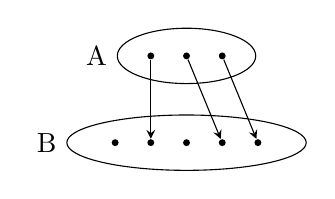
\begin{tikzpicture}
        [
            group/.style={ellipse, draw, minimum height=20pt,
                          minimum width=50pt, label=left:#1},
            dot/.style={circle, fill, minimum width=2.5pt, inner sep=0pt}
        ]
        \node (a) [dot] {};
        \node (b) [dot, right=10pt of a] {};
        \node (c) [dot, right=10pt of b] {};
        \node (q) [dot, below=of a] {};
        \node (r) [dot, below=of b] {};
        \node (s) [dot, below=of c] {};
        \node (p) [dot, left=10pt of q] {};
        \node (t) [dot, right=10pt of s] {};
        \foreach \i/\j in {a/q,b/s,c/t}
            \draw [->, >=stealth,scale=3] (\i) -- (\j);
        \node [fit=(a) (b) (c), group=A] {};
        \node [fit=(p) (q) (r) (s) (t), group=B] {};
    \end{tikzpicture}
    \end{center}
\end{minipage}%
\begin{minipage}[t]{0.50\textwidth}
    \begin{center}
    Surjection\\
    $\forall b \in B.\ \exists a \in A.\ f(a) = b$

    \vspace{15pt}
    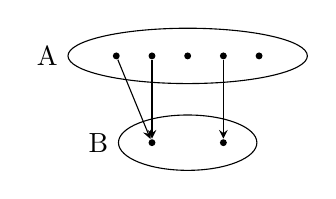
\begin{tikzpicture}
        [
            group/.style={ellipse, draw, minimum height=20pt,
                          minimum width=50pt, label=left:#1},
            dot/.style={circle, fill, minimum width=2.5pt, inner sep=0pt}
        ]
        \node (a) [dot] {};
        \node (b) [dot, right=10pt of a] {};
        \node (c) [dot, right=10pt of b] {};
        \node (d) [dot, right=10pt of c] {};
        \node (e) [dot, right=10pt of d] {};
        \node (p) [dot, below=of b] {};
        \node (q) [dot, below=of d] {};
        \foreach \i/\j in {a/p,b/p,d/q}
            \draw [->, >=stealth,scale=3] (\i) -- (\j);
        \node [fit=(a) (b) (c) (d) (e), group=A] {};
        \node [fit=(p) (q), group=B] {};
    \end{tikzpicture}
    \end{center}
\end{minipage}%
\end{example}


\begin{remark}
    Recall the universal problem of generating a monoid
    $(S^\ast, \epsilon, \cdot)$ from a set $S$ with a function
    $\sigma: S\to S^\ast$. Compare the definition of a universal solution to
    this problem: for all monoids $(M, \shortmid, \star)$,
    \begin{alignat*}{3}
        & \forall\, \text{functions } f:S\to M.\ &&
        \exists!\ \text{homomorphism }
        f^\#: (S^\ast, \epsilon, \cdot)
        \to
        (M, \shortmid, \star)
        .\ &&
        \textcolor{blue}{(}f^\#\textcolor{blue}{) \comp \sigma} = f
        %\\
        %& \forall\, y \in Y.\ &&
        %\exists!\ x \in X.\ &&
        %g(x) = y
    \end{alignat*}
    with the definition of a bijection $g : X \rightarrow Y$:
    \begin{alignat*}{3}
        %& \forall\, \text{functions } f:S\to M.\ &&
        %\exists!\ \text{homomorphism } f^\#:S^* \to M.\ &&
        %f = f^\# \comp \sigma
        %\\
        &
        \forall\, y \in Y.\
        \hspace*{2.5cm}
        &&
        \exists!\ x \in X.\
        \hspace*{5cm}
        &&
        \textcolor{blue}{g(}x\textcolor{blue}{)} = y
    \end{alignat*}

    The similarity suggests that solving an initial universal problem amounts
    to establishing a bijection that \emph{naturally converts} potential
    solutions (in the above example functions between the sets $S$ and $M$) to
    morphisms from the initial universal solution \big(in the above example
    homomorphisms between the monoids $(S^\ast, \epsilon, \cdot)$ and
    $(M, \shortmid, \star)$\big).
    %
    To see this, consider the hom-set of the generated monoid and any other
    monoid $(M, \shortmid, \star)$
    \begin{equation*}
        H_{\catmon}
        = \catmon \big( (S^*, \epsilon, \cdot), (M, \shortmid, \star) \big)
    \end{equation*}
    and the hom-set of our generating set $S$ and the underlying set $M$ of
    the proposed monoid:
    \begin{equation*}
        H_{\catset} = \catset ( S, M )
    \end{equation*}

    The universality condition
    \begin{center}
    \begin{tikzcd}
          S \arrow[r, "\sigma"]  \arrow[rd, swap, "\forall\, f"]
        &
        S^\ast
        \arrow[d, "f^\#"]
        & (S^\ast, \epsilon, \cdot)
        \arrow[d, "\exists!\, f^\# \text{ homomorphism}"]
        \\
        {} & M & (M, \shortmid, \star)
    \end{tikzcd}
    \end{center}
    states that for each function $f \in H_{\catset}$
    we must have a unique $f^\# \in H_{\catmon}$ such that $f = f^\# \comp
    \sigma$.  That is, we must have that the \emph{natural} function
    between $H_{\catmon}$ and $H_{\catset}$ given by
    \begin{equation*}
      \textcolor{blue}{(}-\textcolor{blue}{)\comp\sigma}:
      \catmon \big( (S^*, \epsilon, \cdot), (M, \shortmid, \star) \big)
      %\stackrel\cong
      \longrightarrow
      \catset ( S, M )
    \end{equation*}
    is a bijection.
\end{remark}

\section{Sections and retractions}

\begin{definition}[Sections and retractions]
A \emph{section} $s : A \morpharrow B$ is an arrow for which there exists an
arrow $r : B \morpharrow A$ (a \emph{retraction}) such that
\[
    r \comp s = \id{A}
\]
In other words, a section is the right inverse of some morphism.
Dually, a retraction is the left inverse of some morphism.
\end{definition}

\begin{example}
Consider the category of sets, $\catset$.

\begin{center}
    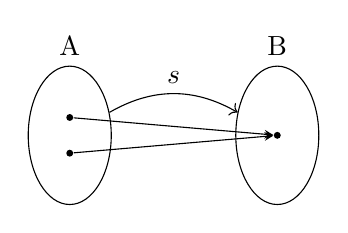
\begin{tikzpicture}
        [
            group/.style={ellipse, draw, minimum height=50pt,
                          minimum width=30pt, label=above:#1},
            dot/.style={circle, fill, minimum width=2.5pt, inner sep=0pt}
        ]
        \node (a) [dot] {};
        \node (b) [dot, below=10pt of a] {};
        \node (p) [dot, xshift=75pt] at ($(a)!1/2!(b)$) {};
        \foreach \i/\j in {a/p,b/p}
            \draw [->, >=stealth,scale=3] (\i) -- (\j);
        \node (A) [fit=(a) (b), group=A] {};
        \node (B) [fit=(p), group=B] {};
        \draw [->] (A) to [bend left] node[above] {$s$} (B);
    \end{tikzpicture}
\end{center}

The above map $s : A \morpharrow B$ can not be a section, as there is no way
to functionally ``go back to two points``.
Hence, a section in $\catset$ must at least be an injection.
However, note that if $A$ is the empty set, $s$ can not be a section.

In $\catset$, $s: A \to B$ is a section iff $s$ is injective and
($A = \emptyset \Rightarrow B = \emptyset$).

A map $r : B \rightarrow A$ is a retraction iff it has a section.
In $\catset$, retractions are the same as surjections (expressed
diagrammatically below).

\begin{center}
    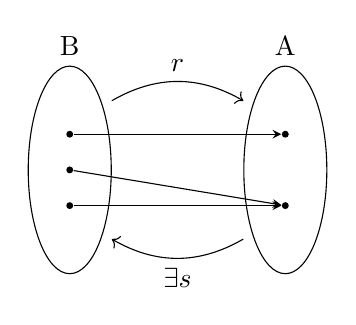
\begin{tikzpicture}
        [
            group/.style={ellipse, draw, minimum height=75pt,
                          minimum width=30pt, label=above:#1},
            dot/.style={circle, fill, minimum width=2.5pt, inner sep=0pt}
        ]
        \node (a) [dot] {};
        \node (b) [dot, below=10pt of a] {};
        \node (c) [dot, below=10pt of b] {};
        \node (p) [dot, right=75pt of a] {};
        \node (q) [dot, right=75pt of c] {};
        \foreach \i/\j in {a/p,b/q, c/q}
            \draw [->, >=stealth,scale=3] (\i) -- (\j);
        \node (B) [fit=(a) (b) (c), group=B] {};
        \node (A) [fit=(p) (q), group=A] {};
        \draw [->] ([yshift=25pt]B.east) to [bend left] node[above] {$r$}
                   ([yshift=25pt]A.west);
        \draw [->] ([yshift=-25pt]A.west) to [bend left] node[below]
                   {$\exists s$} ([yshift=-25pt]B.east);
    \end{tikzpicture}
\end{center}

\end{example}

\subsection{Axiom of choice}
\begin{center}
    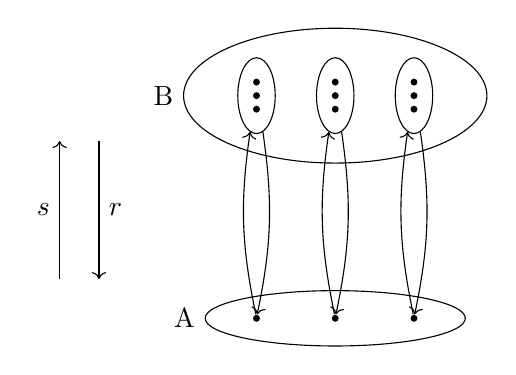
\begin{tikzpicture}
        [
            group/.style={ellipse, draw, minimum height=20pt,
                          minimum width=10pt, label=left:#1},
            dot/.style={circle, fill, minimum width=2.5pt, inner sep=0pt}
        ]
        \foreach \i [count = \xi] in {x,y,z}{
            \node (\i1) [dot] at (\xi, 0) {};
            \node (\i2) [dot,below=2pt of \i1] {};
            \node (\i3) [dot,below=2pt of \i2] {};
            \node (g-\i) [fit=(\i1) (\i2) (\i3), group] {};
            \node (a-\i) [dot] at (\xi, -3) {};
            \draw [->] (g-\i) to [bend left=10] (a-\i);
            \draw [->] (a-\i) to [bend left=10] (g-\i);
        }
        \node (A) [fit=(a-x) (a-y) (a-z), group=A] {};
        \node (B) [fit=(g-x) (g-y) (g-z), group=B] {};
        \draw [->] (-1.5,-2.5) to node[left] {$s$} (-1.5,-0.75);
        \draw [->] (-1.0,-0.75) to node[right] {$r$} (-1.0,-2.5);
    \end{tikzpicture}
\end{center}

The function $r$ has a section if, $\forall a \in A$, we can find a $b \in B$
such that $r(b) = a$.  In other words, $\forall a \in A$, a section $s$ is
defined by choosing $s(a) \in B$ such that $r\big(s(a)\big) = a$.  This may
require the \emph{axiom of choice}.

\begin{definition}
A category $\mathcal{C}$ \emph{satisfies the axiom of choice} whenever every
``surjection'' (technically, \emph{epimorphism}) in $\mathcal{C}$ has a
retraction.
\end{definition}

\section{Injections (technically, \emph{monomorphisms}) in categories}

A function $f : A \rightarrow B$ is \emph{injective} if every element in its
codomain is mapped to by at most one element in its domain:

\begin{equation*}
    \forall a, a' \in A.\ f(a) = f(a') \implies a = a'
\end{equation*}

How could we express this notion categorically? The set-theoretic definition
involves talking about function application and individual \emph{elements} of
sets, which do not in general exist in an arbitrary category. To avoid these
set-specific notions, we attempt to construct a definition which only mentions
morphisms and the operation of morphism composition.

\subsection{Proposed solution 1: morphisms from the terminal object
  (technically, \emph{global elements})}

In the category of sets, there is a bijection between the elements of a set
$S$ and the functions from a singleton set $\setof{*}$ to $S$: mapping $*$ to
an $s \in S$ amounts to selecting the specific element $s$ in $S$. This lets
us abstract over the notion of individual elements and is therefore a good
starting point for generalising the problem to categories. Before that, we
also need a category-theoretic counterpart to singleton sets:
\emph{terminal objects}.

\begin{definition}[Terminal objects]
A \emph{terminal object} in a category $\mathcal C$ is an object $\nelem{1}$
such that
\begin{equation*}
    \forall c \in \Ob(\mathcal C).\ \exists!\, u : c \rightarrow \nelem{1}
\end{equation*}
\end{definition}

A terminal object in $\catset$ is any singleton set, for instance $\{*\}$, as
for every other set $S$ we only have the constant function
$S \rightarrow \{*\}$ mapping $s \in S$ to $*$.
As with all universal constructions, all terminal objects in a category are
isomorphic to each other, so we can talk about \emph{the} terminal object.

Looking back at the definition of injections, we can use the terminal object
of a category to specify two ``elements'' of an object $A$ by as two morphisms
$a$ and $a'$ from $\nelem{1}$ to $A$.

\begin{center}
\begin{tikzcd}
    \nelem{1} \arrow[r, shift left=5pt, "a"]
               \arrow[r,shift right=5pt, swap, "a'"]
    & A \arrow[r, "f"]
    & B
\end{tikzcd}
\end{center}

The application of the function $f$ to the elements $a$ and $a'$ is translated
into composition of the morphisms $a$ and $a'$ with $f$.  We are thus lead to
the following:

\begin{equation*}
    \forall a, a' : \nelem{1} \rightarrow A.\ f \comp a = f \comp a'
    \implies a = a'
\end{equation*}

Unfortunately, this definition is too weak to capture the notion of
``injectivity'' for morphisms: the objects of a category may have internal
structures that cannot be ``selected'' by a morphism from the terminal
object.  Such a category is introduced in Exercise~\ref{lecture-5-exercise}.

\subsection{Proposed solution 2: morphisms from an arbitrary object
  (technically, \emph{generalized elements})}

To fix the issue in the previous definition, we consider mappings from any
object in the category, not just terminal objects.

\begin{definition}
A morphism $f: A\to B$ in a category $\mathcal C$ is said to be a
\emph{monomorphism} whenever
\begin{equation*}
    \forall X \in \Ob(\mathcal C).\
    \forall a, a' : X \rightarrow A \text{ in }\mathcal C.\
      f \comp a = f \comp a' \implies a = a'
    \enspace.
\end{equation*}
\end{definition}

Note how this definition of ``injectivity of morphisms'' (technically
monomorphisms) does not use any set-specific concepts such as elements and
function application: everything is expressed using composition of morphisms
which is available in any category.

\begin{exercise} \label{lecture-5-exercise}
Consider the category of \emph{directed graphs}, $\catdirgraph$:

\begin{itemize}
    \item Objects: tuples $(N, E, s, t)$ where $N$ is the set of nodes, $E$ is
      the set of edges and $s, t : E \rightarrow N$ are functions mapping an
      edge to its source and target nodes respectively.

    \item Morphisms from $G=(N,E,s,t)$ to $G'=(N',E',s',t')$: a pair of
      functions $(\eta, \varepsilon)$, where $\eta : N \rightarrow N'$ maps
      nodes to nodes and $\varepsilon : E \rightarrow E'$ maps edges to edges
      between two graphs such that connectivity is maintained:
      \begin{center}
      \begin{tikzcd}[row sep=0.8em]
      {}
      & E \arrow[ld, swap, "s"] \arrow[dd, "\varepsilon"] \arrow[rd, "t"]
      & {} \\
      N \arrow[dd, swap, "\eta"]
      & {}
      & N \arrow[dd, "\eta"] \\
      {}
      & E' \arrow[ld, "s'"] \arrow[rd, swap, "t'"]
      & {} \\
      N' & {} & N'
\end{tikzcd}
\end{center}
      That is, an
      edge $e$ between nodes $a$ and $b$ in the graph $G$ is mapped to an
      edge $\varepsilon(e)$ between the nodes $\eta(a)$ and $\eta(b)$ in the
      graph $G'$.
\begin{center}
\begin{tikzcd}[row sep=4em]
        a \arrow[r, swap, "e"{name=U}] \arrow[d, dashed, "\eta", mapsto]
      & b \arrow[d, dashed, "\eta"]
      & \text{in $G$}
      \\
        \eta(a) \arrow[r, "\varepsilon(e)"{name=D} , mapsto]
      & \eta(b)
      \arrow[from=U, to=D, dashed, "\varepsilon", mapsto]
      & \text{in $G'$}
\end{tikzcd}
\end{center}
\end{itemize}

What is the terminal object of this category? It contains a single node (as the
singleton set is the terminal object of the set of nodes) and a single looping
edge:

\begin{center}
\begin{tikzcd}
    \bullet \arrow[out=150,in=210, loop, looseness=5]
\end{tikzcd}
\end{center}

In the category $\catdirgraph$, the notion of ``subgraph up to renaming'' is
captured by morphisms $(\eta,\varepsilon)$ such that both $\eta$ and
$\varepsilon$ are injections.
\begin{enumerate}
  \item
    Show that proposed solution 1 is insufficient to characterise the notion
    of subgraph up to renaming.  (Hint: Consider what structures can this
    single loop graph ``select'' from a graph.)
  \item
    Show that proposed solution 2 precisely characterises the notion of
    subgraph up to renaming.
\end{enumerate}
\end{exercise}

\chapter{Functors}
\lecturedetails{24 October 2017}{M Fiore, J Clarke, T Parks}

\section{Duality}
\begin{definition}[Duality]
Given a category $\mathcal{C}$, we define the \emph{opposite} or \emph{dual}
category, $\mathcal{C}^{\mathrm{op}}$, to be the category with:
    \begin{itemize}
        \item $\Ob(\mathcal{C}^{\mathrm{op}}) = \Ob(\mathcal{C})$
        \item $\mathcal{C}^{\mathrm{op}}(A, B) \eqdef \mathcal{C}(B, A)$
    \end{itemize}

\begin{minipage}[t]{0.49\textwidth}
    \begin{center}
        In $\mathcal{C}^{\mathrm{op}}$

        \vspace{15pt}

        \begin{tikzcd}
            A \arrow[d, swap, "f"] \\
            B
        \end{tikzcd}
    \end{center}
\end{minipage}%
\vline%
\begin{minipage}[t]{0.49\textwidth}
    \begin{center}
        In $\mathcal{C}$

        \vspace{15pt}

        \begin{tikzcd}
            A \\
            B \arrow[u, "f"]
        \end{tikzcd}
    \end{center}
\end{minipage}

Identities are the same as in $\mathcal{C}$, that is:

\begin{equation*}
    \id{A}^{\mathrm{op}} \eqdef \id{A}
\end{equation*}

For composition, we need:

\begin{equation*}
    \equalto{\mathcal{C}^{\mathrm{op}}(B, C)}{\mathcal{C}(C, B)} \times
    \equalto{\mathcal{C}^{\mathrm{op}}(A, B)}{\mathcal{C}(B, A)} 
    \xrightarrow{\comp^{\mathrm{op}}_{A,B,C}}
    \equalto{\mathcal{C}^{\mathrm{op}}(A, C)}{\mathcal{C}(C, A)}
\end{equation*}

Therefore, we define:

\begin{equation*}
    g \comp^{\mathrm{op}}_{A,B,C} f = f \comp_{C,B,A} g
\end{equation*}
\end{definition}

\begin{definition}[Monomorphism]
A \emph{monomorphism} in a category $\mathcal{C}$ is a map $f : A \to B$ such
that for all $X \in \Ob(\mathcal{C})$ and for all $a, a' : X \to A$,
$f \comp a = f \comp a' \implies a = a'$.
\end{definition}

\begin{definition}[Epimorphism]
An \emph{epimorphism} in a category $\mathcal{C}$ is a monomorphism in
$\mathcal{C}^{\mathrm{op}}$, \ie~$f : A \to B$ is an epimorphism if:
\[
    \forall T \in \Ob(\mathcal{C}) . \forall t, t' : B \to T .
    t \comp f = t' \comp f \implies t = t'
\]
Here, $T$ can be thought of as an object of ``tests''.
\end{definition}

\begin{exercise}
Show that, in $\catset$, epimorphisms are the same as surjections.
\end{exercise}

\begin{exercise}
Show that each of isomorphisms, epimorphisms, monomorphisms, sections and
retractions are closed under composition; \ie~if $f : A \to B$ and 
$g : B \to C$ are in one of these classes, then so is $g \comp f : A \to C$.
\end{exercise}

\begin{exercise}
Prove the labelled inclusions:

\begin{center}
    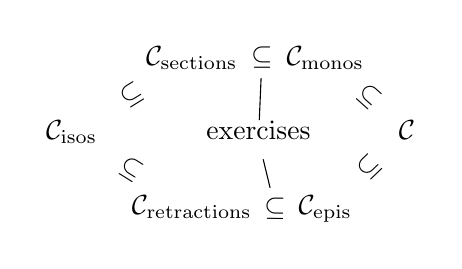
\begin{tikzpicture}
        \matrix[matrix of math nodes, name=m, column sep=0.6em, row sep=1.2em] {
            &
            |[alias=Sec]| \mathcal{C}_{\mathrm{sections}} &
            |[alias=Mono]| \mathcal{C}_{\mathrm{monos}} &
            \\
            |[alias=Cong]| \mathcal{C}_{\mathrm{isos}} &
            |[alias=Ex1]| &
            |[alias=Ex2]| &
            |[alias=C]| \mathcal{C}
            \\
            &
            |[alias=Ret]| \mathcal{C}_{\mathrm{retractions}} &
            |[alias=Epi]| \mathcal{C}_{\mathrm{epis}} &
            \\
        };

        \node (Ex) [fit=(Ex1)(Ex2)]{exercises};

        \path (Cong) edge[draw=none] node[sloped, allow upside down, auto=false] {$\subseteq$} (Sec)
              (Cong) edge[draw=none] node[sloped, allow upside down, auto=false] {$\subseteq$} (Ret)
              (Sec) edge[draw=none] node (SecMono) [sloped, allow upside down, auto=false] {$\subseteq$} (Mono)
              (Ret) edge[draw=none] node (RetEpi) [sloped, allow upside down, auto=false] {$\subseteq$} (Epi)
              (Mono) edge[draw=none] node[sloped, allow upside down, auto=false] {$\subseteq$} (C)
              (Epi) edge[draw=none] node[sloped, allow upside down, auto=false] {$\subseteq$} (C)
              (Ex) edge (SecMono)
              (Ex) edge (RetEpi);
    \end{tikzpicture}
\end{center}
\end{exercise}

Recall that the product of a family of objects $\setof{A_i \suchthat i \in I}$
is given by:

\begin{equation*}
    \left(\prod_{i\in I} A_i\right) \xrightarrow{\pi_k} A_k
    \qquad (k\in I)
\end{equation*}

such that it is a terminal universal solution.

\begin{definition}
\emph{Coproducts}, or \emph{sums}, in $\mathcal{C}$ are products in
$\mathcal{C}^{\mathrm{op}}$. The coproduct of a family
$\setof{A_i \suchthat i \in I}$ is given by

\begin{center}
    \begin{tikzcd}
        A_k \arrow[r, "\iota_k"] \arrow[dr, swap, "\forall f_k"] &
        \left(\coprod_{i \in I} A_i\right) \arrow[d, "\exists!f_k"]
        \\
        &
        X
    \end{tikzcd}
    \qquad$(k\in I)$
\end{center}
\end{definition}

In $\catset$, coproducts are disjoint unions:

\begin{equation*}
    \begin{aligned}
        \coprod_{i \in I} A_i \ = \ \bigcup_{i \in I}\, \setof{i} \times A_i &
        \overset{\iota_k}{\leftarrow} A_k
        \\
        (k, a) &
        \mapsfrom a
    \end{aligned}
\end{equation*}

\begin{exercise}
Calculate coproducts/sums in the categories introduced so far ($\catpfn$,
$\catrel$, $\catpred$, $\catpreo$, $\catmon$, \dots).
\end{exercise}

\begin{exercise}
Prove or disprove whether bijections ($\iffdef$ monomorphic and epimorphic) are
the same as isomorphisms.
\end{exercise}

\section{Functors}

Categories are mathematical structures with their own morphisms,
\emph{functors}:
\begin{center}
\begin{tikzcd}
    \mathcal{A} \arrow[r, "F"]  & \mathcal{B}
\end{tikzcd}
\end{center}
We will motivate their definition by considering two special kinds of
categories, monoids and preorders, together with their respective morphisms.

\subsection{Monoids can be regarded as categories}

A monoid $(M, \shortmid, \star)$ maybe seen as the category $\mathcal M$ with
a single object:
\begin{align*}
\Ob(\mathcal M) &\eqdef \setof{ \bullet }
\end{align*}
for which the hom-set consists of the elements of the monoid:
\begin{align*}
\mathcal{M}(\bullet, \bullet) &\eqdef M
\end{align*}
The identity is the neutral element of the monoid:
\begin{align*}
\id{\bullet} &\eqdef\ \shortmid
\end{align*}
and the composition of morphisms is the monoid multiplication:
\begin{align*}
f \comp g &\eqdef f \star g
\enspace.
\end{align*}

Conversely, every category $\mathcal C$ with a singleton set of objects, say
$\setof{\bullet}$, has an underlying monoid structure given by 
\[
  \big(\, \mathcal{C}(\bullet,\bullet) \,,\, \id{\bullet} \,,\, \comp \,\big) 
\]

The above two constructions are in bijective correspondence.

\subsection{Preorders can be regarded as categories}

For a preorder $(P, \leq)$, consider the category $\mathcal P$ with
$\Ob(\mathcal P) = P$ and hom-sets
\[
\mathcal{P}(p, q) 
= \begin{cases}
    \bigsetof{\, (p,q) \,} & \text{if } p \leq q
    \\[1mm]
    \emptyset & \text{otherwise }
  \end{cases}
\qquad
(p,q \in P)
\]

As $p \leq p$, the identity is given by
\begin{align*}
\id{p} &\eqdef (p,p)
\end{align*}

We also need to consider the operation of composition:
\[
\mathcal{P}(q, r) \times \mathcal{P}(p, q) \to \mathcal{P}(p, r)
\]
We can determine it by cases: 
\begin{itemize}
\item
If either $\mathcal{P}(q, r)$ or $\mathcal{P}(p, q)$ are empty, then so is 
$\mathcal{P}(q, r) \times \mathcal{P}(p, q)$ and the composition map is
uniquely determined.

\item
Otherwise, both $\mathcal{P}(q, r)$ and $\mathcal{P}(p, q)$ are singleton
sets so that, by the transitivity property of preorders, so is 
$\mathcal{P}(p, r)$; and the composition map is again uniquely determined.
\end{itemize}

Conversely, every category $\mathcal C$ with a set of objects and
subsingleton~(\viz,~a subset of a singleton) hom-sets has an underlying
preorder structure given by 
\[
  \big(\, \Ob(\mathcal C) \,,\, \leq \,\big)
\]
where $X \leq Y \iffdef ( \mathcal{C}(X, Y) \iso \nelem 1 )$.

\paragraph{Locally small and small categories.}
%
The notion of category we have considered, with a class of objects and
hom-sets, is technically referred to as \emph{locally small}.  Categories with
a set of objects are referred to as \emph{small}.  The categories associated
to monoids and preorders are small.

\subsection{Morphisms of monoids, preorders, and categories}

We recall the notions of morphism between monoids and preorders, and
generalize them to categories.

\begin{center}\begin{tabular}{ccc}
Monoids and homomorphisms & \qquad\qquad\qquad & Preorders and monotone
functions
\\[3mm]
$(M_1, \shortmid_1, \star_1) 
 \stackrel{h}{\longrightarrow} 
 (M_2, \shortmid_2, \star_2)$ 
&& 
$(P_1, \leq_1) \stackrel{f}{\longrightarrow} (P_2, \leq_2)$       
\\[3mm]
\begin{tabular}{l}
$h: M_1 \to M_2$                               
\\[1mm]
s.t.~$h(\shortmid_1) =\ \shortmid_2$ 
\\[1mm]
\phantom{s.t.~}$h(x \star_1 y) = h(x) \star_2 h(y)$   
\end{tabular}
&& 
\begin{tabular}{l}
$f: P_1 \to P_2$ 
\\[1mm]
s.t.~$p \leq_1 q \implies f(p) \leq_2 f(q)$ 
\end{tabular}
\end{tabular}
\end{center}

\begin{center}\begin{tabular}{c}
Categories and functors
\\[3mm]
$\mathcal{C}_1 \stackrel{F}{\longrightarrow} \mathcal{C}_2$                
\\[4mm]
$\left\{
\begin{array}{l}
F_{\textrm{obj}} : \Ob(\mathcal{C}_1) \to \Ob(\mathcal{C}_2)
\\[3mm]
F_{\textrm{arr}} : \Arr(\mathcal{C}_1) \longrightarrow \Arr(\mathcal{C}_2)
\end{array}
\right.$
\\[8mm]
\begin{tabular}[t]{lc}
s.t. &
\\
&
% the yshift is needed to make the F_arrow level.
\begin{tikzcd}
P 
\arrow[dd, "f"{name=L, right}] & & F_{obj}(P) 
\arrow[dd, "F_{\text{arr}}(f)"{name=R, left}] 
\\
\arrow[rr, "F_{arr}", from=L, to=R, start anchor={[yshift=-0.2ex]}, mapsto] 
&  &  
\\
Q &  & F_{obj}(Q)
\end{tikzcd}
\\[20mm]
&
$F_{\textrm{arr}}( \id{X} ) \,=\, \id{ F_{\textrm{obj}}(X) }$ 
\\[6mm]
&
\begin{tikzcd}
A \arrow[d, "f"] \arrow[dd, "g \comp f"', bend right=50] 
&  
F_\text{obj}(A) 
\arrow[d, "F_\text{arr}(f)"{left}] 
\arrow[dd, "F_\text{arr}(g \comp f)", bend left=55] 
\\
B \arrow[d, "g"] & F_\text{obj}(B) \arrow[d, "F_\text{arr}(g)"{left}] 
\\
C & F_\text{obj}(C)
\end{tikzcd}
\end{tabular}
\end{tabular}\end{center}

\chapter{Natural transformations}
\lecturedetails{26 October 2017}{M Fiore, \ldots}

\end{document}
